\documentclass{article}
\usepackage[utf8]{inputenc}
\usepackage[T1]{fontenc}
\usepackage[frenchb]{babel}
\usepackage{soul}
\usepackage{graphicx}
\usepackage{float}

% Faire l'algo de tri par dichotomie

\title{Enregistrement}

\begin{document}
Modèle\newline
Cette partie de l'application est principalement basée sur l'analyse et l'enregistrement des notes jouées par 
l'utilisateur. Le principe est d'analyser en temps réel les fréquences à la base du son de la guitare, et de faire en sort de constituer un accord
avec les notes ayant le volume le plus fort et l'enregistrer. De plus, le modèle comporte également toutes les informations sur les préférences
de l'utilisateur pour l'application,   ainsi que des fonctions pour enregistrer les données. Nous avons choisi de sauvegarder les fichiers au format JSON.\newline

UML du modèle de l'application:
\begin{figure}[H]
\centering
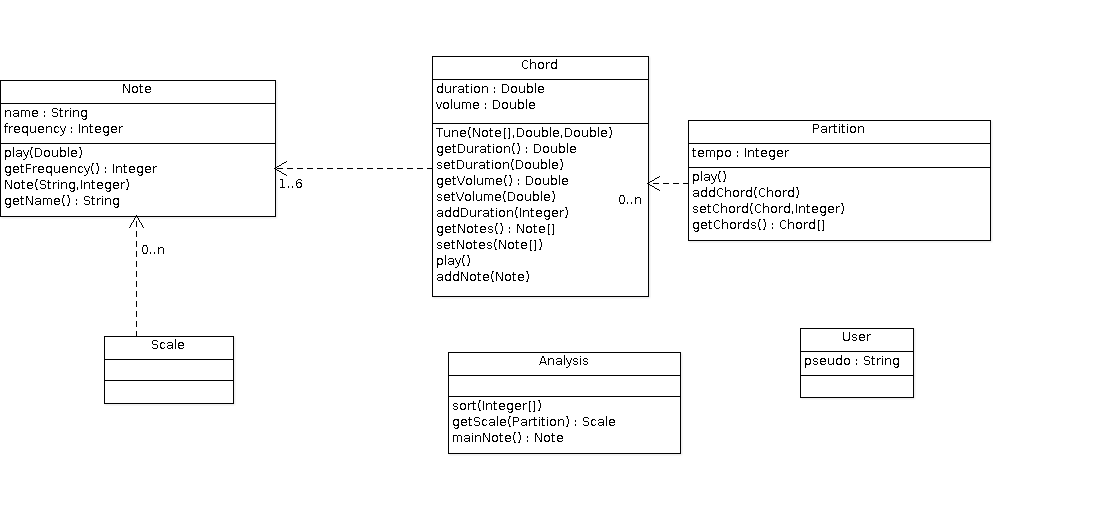
\includegraphics[scale=0.5]{ModelUML}
\caption{UML du modele}
\end{figure}

La classe Note représente une Note qui n'est pas jouée, c'est-à-dire qu'elle contient la définition d'une note seulement.\newline
La classe Chord permet donc de représenter de 1 à 6 note jouée simultanément tel un accord à la guitare.\newline
La classe Partition représente donc une partition comme l'utilisateur va la voir.\newline
La classe Analysis propose différentes fonctions essentielles à l'application. Cette classe propose également des fonctionnalités pour l'apprentissage de la composition de musiques.\newline
La classe Scale représente une gamme. Une gamme est une suite de notes, et la classe est donc composée d'un certain nombre de note.
La classe User est présente pour enregistrer le pseudonyme de l'utilisateur pour pouvoir envoyer des partitions sur le site.
Lorsque l'utilisateur va jouer une note, le logiciel va récupérer toutes les fréquences entrant par le micro et les trier en fonction de leur volume. Il est donc aisé par la suite de trouver quelles sont les notes qui sont le plus jouées.


\begin{figure}[H]
\centering
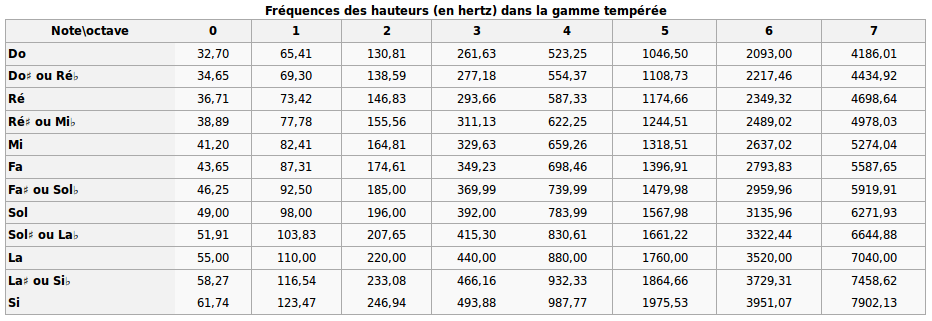
\includegraphics[scale=0.5]{Frequences}
\caption{Toutes les frequences possibles}
\end{figure}


\begin{tabbing}

\ul{fonction} analyser(frequences : \ul{tableau entier}[0..n], n : \ul{entier}, seuilMin : \ul{entier}) : \ul{tableau Accord}\\
\ul{debut}\\
frequences <- trier(frequences)\\
i <- 0\\
complet <- faux\\
\ul{Tant que} i < n \ul{et} \ul{non} complet \ul{faire}\\
    freq <- frequences[i]\\
    \ul{Si} freq > seuilMin \ul{et} \ul{non} present(retour, freq)\\
    \ul{alors}\\
        ajouter(retour, freq)\\
        \ul{Si} taille(retour) > 5\\
        \ul{alors}\\
            complet <- vrai\\
        \ul{fsi}\\
    \ul{fsi}\\
\ul{ftantque}\\
\ul{retourne} retour\\
\ul{fin}\\
\end{tabbing}

% Algo de récupérer une note avec sa fréquence
\begin{tabbing}
\ul{fonction} recupererNote(frequence : \ul{entier}, notes : \ul{Note[0..n]}, n : \ul{entier}) : Note\\
\ul{debut}\\
min <- 0\\
max <- n\\
trouve <- faux\\
\ul{Tant que} min <= max \ul{et} \ul{non} trouve \ul{faire}\\
    indice <- (max + min) /2 \\
    frequenceNote <- notes[indice].frequence\\
    \ul{Si} frequence = frequenceNote\\
    \ul{alors}\\
        retour <- notes[indice]\\
        trouve <- vrai\\
    \ul{sinon}\\
        \ul{Si} frequence < frequenceNote\\
        \ul{alors}\\
            max <- indice\\
        \ul{sinon}\\
            min <- indice\\
        \ul{fsi}\\
    \ul{fsi}\\
\ul{ftantque}\\
\ul{Si} \ul{non} trouve\\
\ul{alors}\\
    retour <- notes[min]\\
\ul{fsi}\\
\ul{retourne} retour\\
\ul{fin}\\
\end{tabbing}


\begin{tabbing}
\ul{fonction} trier(frequences : \ul{tableau eniter}[0..n], n\ul{entier})
\end{tabbing}


\begin{tabbing}
\ul{fonction} montrerNote(mic : \ul{entreeMicro})\\
\ul{debut}\\
accorder <- vrai\\
\ul{Tant que}\\
freqs <- recupererFrequences(mic)\\
freqs <- trier(freqs)\\
\ul{ecrire} recupererNote(freqs[0])\\
\ul{ftantque}\\
\ul{fin}\\
\end{tabbing}

%Enregistrement d'une partition
\begin{tabbing}
\ul{fonction} enregistrer(mic : \ul{entreeMicro}, seuilHaut :  \ul{entier}, seuilBas : \ul{entier}, tempo : \ul{entier}) : \ul{Partition}\\
\ul{debut}\\
enregistrer <- vrai\\
j <- 0\\
\ul{Tant que} enregistrer \ul{faire}\\
    frequences <- recupererFrequences(mic)\\
    frequences <- trier(frequences)\\
    complet <- faux\\
    fini <- faux\\
    i <- 0 \\
    \ul{Tant que} \ul{non} complet \ul{et} \ul{non} fini \ul{faire}\\
        frequence <- frequences[i]
        \ul{si} frequence > seuilHaut\\
        \ul{alors}\\
            ajouter(freqs, accord)\\
            j <- j + 1\\
        \ul{sinon}\\
            \ul{si} frequence > seuilBas\\
            \ul{alors}\\ 
                ajouterTemps(retour[j], tempo / 16)\\
            \ul{sinon}\\
                fini <- vrai\\
        \ul{fsi}
    \ul{ftantque}\\     
    i <- i + 1\\  
    attendre(tempo / 16)\\
\ul{ftantque}\\
\ul{retourne} retour \\
\ul{fin}\\
\end{tabbing}

Nous attendons pendant tempo / 16 car c'est la plus petite unité de temps représentable dans une partition. L'utilisateur doit rentrer le tempo dans lequel il compte jouer.

\end{document}